%
% antennenAllgemein.tex 
%
% 
%
% !TEX root = ../../buch.tex
% !TEX encoding = UTF-8
%

\section{Antennen\label{antennen:antennenAllgemein}}
\rhead{Antennen}

Antennen sind in der heutigen technologisch geprägten Welt nicht mehr weg zu denken. Sie befinden sich in vielen verschiedenen Arten und Formen in unseren elektronischen Geräten. Eine Antenne wandelt grundsätzlich die in einer Leitung geführte gebundene elektromagnetische Welle in eine freie Welle im Raum um. Da eine Antenne freie Wellen ebenso in gebundene leitungsgeführte Wellen umwandeln kann hat sie reziproke Eigenschaften.

Eine genauere Erklärung von elektromagnetischen Wechselwirkungen kann sich im \href{buch:chapter:maxwell}{Kapitel Maxwell},
welches sich mit den Maxwell Gleichungen befasst, angeeignet werden. 
\subsection{Loop-Antennen\label{antennen:antennenAllgemein_loop}}
\rhead{Loop-Antennen}

Eine Loop-Antenne hat eine simple Funktionsweise. Sie besteht aus einem Stück Draht wie in Abbildung \ref{antennen:loopAntenne} dargestellt. Die Loop-Antenne kann, nicht wie der Name impliziert, verschiedenste Formen annehmen. Durch den Leiter wird ein Signal geführt, das in der aufgespannten Fläche ein magnetisches Feld induziert. Dieses Feld wird durch Anpassung der Signalamplitude verändert. Eine solche Änderung kann als Information angesehen werden, die sich nun im freien Raum fortbewegt.

\definecolor{conductorYellow}{HTML}{ffc000}
\definecolor{cableBlue}{HTML}{00b0f0}
\def\opening{3}
\def\arcRadius{1.5}
\def\wirelen{10.5}
\def\wireampl{0.8}
\begin{figure}
	\centering
	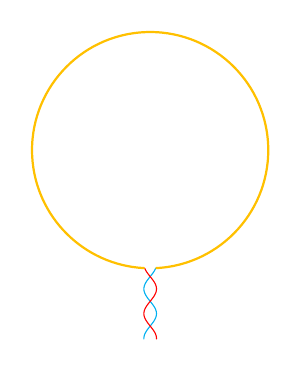
\begin{tikzpicture}[scale=1]
	\begin{scope}[scale=0.1]
		\draw[shift={(-\wireampl+0.02,-\wirelen)}, rotate=90, 
		color=cableBlue, cap=round] plot[domain=1.5:\wirelen, 
		samples=100] (\x, {sin(\x r)*\wireampl});
	\end{scope}
	
	\begin{scope}[scale=0.1]
		\draw[shift={(-\wireampl+0.02,-\wirelen)}, rotate=90, 
		color=red, cap=round] plot[domain=1.5:\wirelen, 
		samples=100] (\x, {sin(\x r)*-\wireampl});
	\end{scope}
	
	\draw[color=conductorYellow, thick, cap=round](0,0)  
	arc[start angle=-90+\opening), end angle=(270-\opening), radius=\arcRadius];
	\end{tikzpicture}
	\caption{Form einer typischen Loop-Antenne}
	\label{antennen:loopAntenne}
\end{figure}

\subsection{Eigenschaften\label{antennen:antennenEigenschaften}}
\rhead{Eigenschaften}
Der Wirkungsgrad
\begin{equation}
	\eta=\frac{P\textsubscript{rad}}{P\textsubscript{tot}},
	\label{antennen:Wirkungsgrad}
\end{equation}
auch Effizienz genannt, kann mittels der Gesamtleistung der Antenne $P\textsubscript{tot}$ und der abgestrahlten Leistung $P\textsubscript{rad}$ berechnet werden. Eine Leistung $P$ entspricht dem elektrischen Widerstand multipliziert mit der Stromstärke im Quadrat. Nach Vereinfachung ergibt sich, dass die Effizienz

\begin{equation}
	\eta=\frac{P\textsubscript{rad}}{P\textsubscript{tot}}=\frac{R\textsubscript{rad}\cdot{I^2}}{R\textsubscript{tot}\cdot{I^2}}=\frac{R\textsubscript{rad}\cdot{I^2}}{(R\textsubscript{rad}+R\textsubscript{loss})\cdot{I^2}}=\frac{R\textsubscript{rad}}{R\textsubscript{rad}+R\textsubscript{loss}}
	\label{antennen:Wirkungsgradkomplett}
\end{equation}
nur noch vom Verlustwiderstand und dem Strahlungswiderstand abhängig ist. $R\textsubscript{rad}$ und $R\textsubscript{loss}$ werden wie folgt definiert:
\begin{align}
	R_{\text{rad}} &= 31171 \Omega \cdot \bigg( \frac{A}{\lambda^2} \bigg)^2 \tag{20.3} \label{antennen:Rrad} \\
	R_{\text{loss}} &= \frac{\rho \cdot l}{r^2 \cdot \pi} \tag{20.4} \label{antennen:Rloss}
\end{align}

Die Formel für die Berechnung des Strahlungswiderstands \eqref{antennen:Rrad} wurde aus Fachliteratur, spezifischer aus dem Buch ``Antenna Theory'' von Constantine A. Balanis, übernommen \cite{antennen:antennaTheory}. Diese gilt für die verschiedensten Formen von Loop-Antennen, welche einen kleinen Umfang  $l$ < $\lambda$/10 aufweisen. $A$ wird hierbei als aufgespannte Fläche definiert, während $\lambda$ der Wellenlänge entspricht. Eine Wellenlänge 
\setcounter{equation}{4}

\begin{equation}
	\lambda = \frac{c}{f}
	\label{antennen:lambda}
\end{equation}
entspricht dem Verhältnis der materialspezifischen Lichtgeschwindigkeit $c$ und der Einsatzfrequenz $f$.
Der Verlustwiderstand wird aus dem spezifischen Widerstand $\rho$, dem Umfang $l$ und dem Leiterradius $r$ berechnet. Die Formeln \eqref{antennen:Rrad} und \eqref{antennen:Rloss} können in dieser Arbeit vereinfacht werden, da die Einsatzfrequenz und die Drahteigenschaften als konstant und gegeben angesehen werden können. Es resultieren die Ausdrücke 
\begin{align}
	R_{\text{rad}} &= k_{\text{1}} \cdot A^2 \tag{20.6} \label{antennen:Rrad_konst} \\
	R_{\text{loss}} &= k_{\text{2}} \cdot l \tag{20.7} \label{antennen:Rloss_konst}
\end{align}
für die beiden Widerstände. $k\textsubscript{1}$ und $k\textsubscript{2}$ werden als Konstanten betrachtet. Eingesetzt in \eqref{antennen:Wirkungsgradkomplett} ergibt sich
\setcounter{equation}{7}
\begin{equation}
	\eta=\frac{k\textsubscript{1}\cdot{A^2}}{k\textsubscript{1}\cdot{A^2}+{k\textsubscript{2}\cdot{l}}}=\frac{1}{1+\frac{k\textsubscript{2}\cdot{l}}{k\textsubscript{1}\cdot{A^2}}}
	\label{antennen:Wirkungsgradeingesetzt}
\end{equation}
als Formel für den Wirkungsgrad.
